\begin{tiny}(Ccp09)\end{tiny}
\begin{figure}[h]
 \centering
 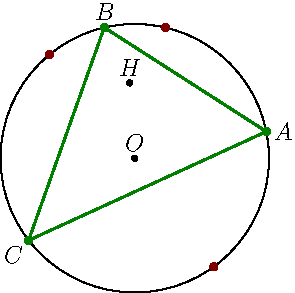
\includegraphics[width=4cm]{./Ccp09_1.pdf}
 \caption{Exercice \arabic{enumi}}
 \label{fig:Ccp09_1}
\end{figure}

\begin{enumerate}
 \item Pour montrer que $H$ est sur la hauteur issue de $A$, il suffit de vérifier que 
\begin{displaymath}
 \frac{h -a}{b-c} \in i\R
\end{displaymath}
Comme $b$ et $c$ sont de module $1$ leur inverse est égal à leur conjugué donc
\begin{multline*}
 \frac{h -a}{b-c} = \frac{b+c}{b-c}
 = \frac{1}{|b-c|^2}(b+c)(\frac{1}{b}-\frac{1}{c})\\
 = \frac{1}{|b-c|^2}(\frac{c}{b}-\frac{b}{c})
 = \frac{1}{|b-c|^2}(c\overline{b}-b\overline{c})\\
 = 2i \frac{\Im(c\overline{b})}{|b-c|^2}\in i\R
\end{multline*}

Les autres orthogonalités se traitent dela même manière. On remarque la permutation circulaire des lettres $a$, $b$, $c$.

 \item Exprimons les 6 différences avec $\frac{h}{2}$. Elles sont respectivement égales à:
\begin{displaymath}
 \frac{a}{2},\,\frac{b}{2},\,\frac{c}{2},\,\frac{a}{2},\,\frac{b}{2},\,\frac{c}{2}   
\end{displaymath}
donc de même module $\frac{1}{2}$. Les 6 points sont sur le cercle de centre de point d'affixe $\frac{h}{2}$ et de rayon $\frac{1}{2}$.
 
 
 \item Calculons l'affixe du symétrique de $H$ par rapport à la droite $(BC)$ avec l'expression de la symétrie trouvée dans l'exercice \ref{Ecp40}.
\begin{multline*}
 s_{(BC)}(h) = -bc(\overline{a+b+c}+b+c\\
 = -\frac{bc}{a} -c -b + b + c = -\frac{bc}{a} 
\end{multline*}

Par permutation circulaire, on trouve des quatients analogues pour les autres symétriques. Ils sont tous de module $1$. Ces 3 symétriques sont sur le cercle unité contenant les points $A$, $B$, $C$.
\end{enumerate}
